% !TeX program = xelatex
% 连续运行两次 XeLaTeX，以生成完整目录和交叉引用。
\documentclass[UTF8,a4paper,zihao=-4,fontset=none]{ctexart}
\usepackage[margin=2.5cm,headheight=16pt]{geometry}
\usepackage{fontspec}
\setmonofont{DejaVu Sans Mono}[Scale=MatchLowercase]
\setCJKmainfont{Noto Serif CJK SC}
\setCJKsansfont{Noto Sans CJK SC}
\setCJKmonofont{Noto Sans Mono CJK SC}
\usepackage{amsmath,amssymb,booktabs,array,longtable,graphicx}
\usepackage{xcolor,fancyhdr,caption,hyperref,fvextra,float,enumitem}
\definecolor{navy}{HTML}{173B59}
\definecolor{softgray}{HTML}{F4F6F8}
\hypersetup{colorlinks=true,linkcolor=navy,urlcolor=navy,citecolor=navy,
  pdftitle={编程作业三：基于解码器语言模型的文本分类},
  pdfsubject={分类头微调、朴素贝叶斯与 Prompt 范式对比}}
\captionsetup{font=small,labelfont=bf,labelsep=quad}
\ctexset{section={format=\Large\bfseries\sffamily\color{navy}},
  subsection={format=\large\bfseries\sffamily}}
\setlength{\parindent}{2em}
\linespread{1.25}
\setlength{\emergencystretch}{2em}
\setlist{nosep,leftmargin=2em}
\renewcommand{\topfraction}{0.92}
\renewcommand{\bottomfraction}{0.85}
\renewcommand{\textfraction}{0.05}
\renewcommand{\floatpagefraction}{0.8}
\makeatletter
\setlength{\@fptop}{0pt}
\setlength{\@fpsep}{12pt}
\setlength{\@fpbot}{0pt plus 1fil}
\makeatother
\pagestyle{fancy}
\fancyhf{}
\fancyhead[L]{\small 编程作业三：文本分类}
\fancyhead[R]{\small 实验报告}
\fancyfoot[C]{\thepage}
\renewcommand{\headrulewidth}{0.4pt}
\newcommand{\code}[1]{\texttt{\small\detokenize{#1}}}
\DefineVerbatimEnvironment{CodeBlock}{Verbatim}{fontsize=\small,breaklines=true,
  frame=single,rulecolor=\color{gray!40},framesep=2mm}
% 本文件由 scripts/report_values.py 自动生成，请勿手工修改。
\newcommand{\DatasetTrain}{108,000}
\newcommand{\DatasetValidation}{12,000}
\newcommand{\DatasetTest}{7,600}
\newcommand{\VocabSize}{30,000}
\newcommand{\MeanTokens}{47.83}
\newcommand{\MedianTokens}{46}
\newcommand{\TokenPnn}{108}
\newcommand{\MaxTokens}{314}
\newcommand{\TruncatedTrainPct}{0.066}
\newcommand{\TruncatedTestPct}{0.053}
\newcommand{\LMParams}{10,888,704}
\newcommand{\LMInitLoss}{10.3450}
\newcommand{\LMFinalLoss}{3.9327}
\newcommand{\LMInitVal}{10.3449}
\newcommand{\LMFinalVal}{4.0634}
\newcommand{\LMInitPpl}{31,099.48}
\newcommand{\LMFinalPpl}{58.17}
\newcommand{\LMTrainSeconds}{104.97}
\newcommand{\LMTokens}{24,576,000}
\newcommand{\LMStreamTokens}{5,380,808}
\newcommand{\LMPeakMiB}{4,673}
\newcommand{\FullAcc}{93.24}
\newcommand{\FullFOne}{93.22}
\newcommand{\FullValAcc}{93.50}
\newcommand{\FullTrainable}{10,889,732}
\newcommand{\FullTotal}{10,889,732}
\newcommand{\FullBackbone}{10,888,704}
\newcommand{\FullHead}{1,028}
\newcommand{\FullTrainSeconds}{94.68}
\newcommand{\FullInferSeconds}{0.63}
\newcommand{\FullThroughput}{11,990}
\newcommand{\FullBestEpoch}{3}
\newcommand{\FullPeakMiB}{1,200}
\newcommand{\FrozenAcc}{88.03}
\newcommand{\FrozenFOne}{88.02}
\newcommand{\FrozenTrainable}{1,028}
\newcommand{\FrozenTrainSeconds}{71.75}
\newcommand{\FrozenThroughput}{12,296}
\newcommand{\FrozenBestEpoch}{6}
\newcommand{\ScratchAcc}{91.86}
\newcommand{\ScratchFOne}{91.83}
\newcommand{\ScratchTrainSeconds}{94.34}
\newcommand{\ScratchThroughput}{12,191}
\newcommand{\NBAcc}{90.57}
\newcommand{\NBFOne}{90.53}
\newcommand{\NBValAcc}{91.03}
\newcommand{\NBAlpha}{0.1}
\newcommand{\NBFeatures}{200,000}
\newcommand{\NBParams}{800,004}
\newcommand{\NBTrainSeconds}{6.85}
\newcommand{\NBFeatureSeconds}{6.83}
\newcommand{\NBInferSeconds}{0.2804}
\newcommand{\NBThroughput}{27,102}
\newcommand{\NBCrossAgreement}{100.0}
\newcommand{\PromptAcc}{73.24}
\newcommand{\PromptFOne}{72.94}
\newcommand{\PromptDefaultAcc}{48.61}
\newcommand{\PromptFewAcc}{63.57}
\newcommand{\PromptFewFOne}{60.20}
\newcommand{\PromptInferSeconds}{3.08}
\newcommand{\PromptThroughput}{2,468}
\newcommand{\PromptTunedVal}{73.21}
\newcommand{\PromptTuningCombos}{72}
\newcommand{\PromptShotsTokens}{108}
\newcommand{\ComparisonBest}{解码器全参数微调}
\newcommand{\SampleCount}{3}
\newcommand{\Seed}{42}
\newcommand{\TorchVersion}{2.6.0+cu124}
\newcommand{\PythonVersion}{3.12.9}
\newcommand{\GPU}{NVIDIA GeForce RTX 3090}
\newcommand{\CUDAVersion}{12.4}
\newcommand{\FullLoss}{0.2166}
\newcommand{\PromptSelectedWorld}{politics}
\newcommand{\PromptSelectedSports}{sports}
\newcommand{\PromptSelectedBusiness}{financial}
\newcommand{\PromptSelectedSciTech}{computers}


\begin{document}
\thispagestyle{plain}
\begin{center}
{\small\color{gray} 编程作业三\quad 实验报告}\par
\vspace{0.5em}
{\zihao{2}\bfseries 基于解码器语言模型的文本分类}\par
\vspace{0.25em}
{\large 分类头微调、朴素贝叶斯与 Prompt 范式对比}\par
\vspace{0.8em}
{\small 人智2401班}\par
\vspace{0.35em}
{\small
\renewcommand{\arraystretch}{1.2}
\begin{tabular}{@{}l@{\hspace{2.2em}}l@{}}
石皓文\enspace 2233316022 & 张恩瑞\enspace 2244413862\\
杜鹏宇\enspace 2223210437 & 许程\enspace 2244313744
\end{tabular}
}\par
\vspace{0.5em}
{\color{gray!50}\rule{0.92\textwidth}{0.4pt}}
\end{center}
\begin{abstract}
复用编程作业二手写的因果多头注意力、LayerNorm 和 Pre-LN 解码器，在 AG News
四分类数据集上完成三种文本分类方案：线性分类头微调、词袋多项式朴素贝叶斯基线
和 Prompt 打分。全参数微调的测试准确率为 \FullAcc\%，
随机初始化同结构模型为 \ScratchAcc\%，朴素贝叶斯为 \NBAcc\%，
冻结主干的线性探针为 \FrozenAcc\%，校准后的零样本 Prompt 为 \PromptAcc\%。
分类头共 \FullHead{} 个参数；Prompt 无可训练参数，准确率低于监督方案。
报告记录数据划分、参数统计、训练开销、样例输出、调试过程和方案分析。
\end{abstract}
\noindent\textbf{关键词：}文本分类；解码器语言模型；分类头；朴素贝叶斯；Prompt；AG News

\tableofcontents
\newpage

\section{任务与方案概览}

本次作业在作业二解码器语言模型的基础上完成文本分类，要求保留手写主干，并比较
至少两种方案。本实验实现三种方案：
\begin{enumerate}
  \item \textbf{微调式分类器}：在解码器最后一层隐状态上取最后一个有效词元，
        接单层线性分类头，用交叉熵训练；支持冻结主干与全参数微调两种模式，
        并额外做随机初始化消融。
  \item \textbf{多项式朴素贝叶斯}：使用同一套小写正则分词，统计 unigram + bigram
        词袋，显式实现拉普拉斯平滑、对数先验和线性判别，并用 sklearn 的
        \code{MultinomialNB} 交叉核对。
  \item \textbf{Prompt 范式}（选做）：构造英文模板，把类别映射为
        \code{politics} / \code{sports} / \code{financial} / \code{computers} 等 verbalizer，直接用语言模型
        给类别词打分；实现零样本与四样本两种设置，并加入 content-free 上下文校准。
\end{enumerate}
所有实验使用同一份 AG News 划分、同一分词器和同一测试集。主结果由脚本
从原始日志和预测文件汇总，报告数字通过 \code{scripts/report_values.py} 注入。

\section{数据集、分词与实验环境}

\subsection{AG News 数据集}
AG News 是公开英文新闻主题分类数据集\cite{zhang2015}，四类为
World、Sports、Business、Sci/Tech。实验使用公开 CSV 镜像
\url{https://github.com/mhjabreel/CharCnn_Keras/tree/master/data/ag_news_csv}：
官方训练集 120,000 条，官方测试集 7,600 条。本实验从官方训练集按类别分层抽取
10\% 作为验证集，得到 \DatasetTrain{} 条训练、\DatasetValidation{} 条验证、
\DatasetTest{} 条测试；测试集仅用于最终评估。
表~\ref{tab:data} 给出类别分布。

\begin{table}[htbp]
\centering\small
\caption{AG News 数据划分与类别分布}\label{tab:data}
\begin{tabular}{lrrrr}
\toprule
分区 & World & Sports & Business & Sci/Tech \\
\midrule
训练集 & 27,000 & 27,000 & 27,000 & 27,000 \\
验证集 & 3,000 & 3,000 & 3,000 & 3,000 \\
测试集 & 1,900 & 1,900 & 1,900 & 1,900 \\
\bottomrule
\end{tabular}
\end{table}

每条样本按 \code{title + ". " + description} 拼接，标题在前；正文仅做小写化
和正则分词，保留 Reuters 模板、URL 片段等原始内容，以保持公开数据的原始分布。
数据文件与划分记录的 SHA-256 保存在 \code{data/metadata.json}。

\subsection{词级分词器}
作业二使用字符级词表。AG News 一条新闻平均约 48 个词，若继续按字符编码，
192 个位置只能覆盖很短的文本，分类和 Prompt 都会严重截断。因此本实验把作业二
仅在训练集建词表的做法扩展到词级：
\begin{itemize}
  \item 小写化后按“单词（允许内部撇号）或单个非空白标点”的正则切分，
        标点单独成词；
  \item 只在 \DatasetTrain{} 条训练文本上统计词频，保留频次不小于 2 的词，
        词表上限 \VocabSize{}；
  \item 加入 \code{<pad>/<unk>/<bos>/<eos>} 四个特殊词元，以及模板词
        \code{topic/title/description} 和两套类别 verbalizer，使 Prompt
        打分时类别词保留在词表中；
  \item 训练语言模型时，文档之间插入 \code{<bos>/<eos>}，再从拼接流中随机
        截取连续窗口做下一个词预测。
\end{itemize}
表~\ref{tab:length} 给出训练集词元长度统计，最长样本 \MaxTokens{} 个词元。
分类和语言模型的上下文长度均取 192，仅截断约 \TruncatedTrainPct\% 的训练样本
和 \TruncatedTestPct\% 的测试样本，绝大多数新闻可以完整覆盖。

\begin{table}[htbp]
\centering\small
\caption{训练集词元长度统计（小写正则分词）}\label{tab:length}
\begin{tabular}{lrrrrr}
\toprule
均值 & 中位数 & P90 & P99 & 最大值 & 超过 192 的比例 \\
\midrule
\MeanTokens & \MedianTokens & 63 & \TokenPnn & \MaxTokens & \TruncatedTrainPct\% \\
\bottomrule
\end{tabular}
\end{table}

\subsection{运行环境}
实验在单张 NVIDIA RTX 3090（24 GiB）上完成，软件环境为 Python \PythonVersion、
PyTorch \TorchVersion、CUDA \CUDAVersion、scikit-learn 1.6.1、NumPy 2.2.4。
随机种子固定为 \Seed，参数和优化器状态使用 FP32，GPU 前向使用 BF16 autocast；
确定性算法开启，cuBLAS workspace 固定，以保证训练可复现。
语言模型预训练、分类微调和 Prompt 推理均记录实际耗时与 CUDA 峰值显存。

\section{方法}

\subsection{复用的手写解码器主干}
词表大小为 $V$，上下文长度为 $T_{\max}$，隐藏维度为 $d$，层数为 $L$。
输入词元 $X\in\{0,\ldots,V-1\}^{B\times T}$ 先经过词嵌入和可学习绝对位置嵌入：
\begin{equation}
H^{(0)}_{b,t}=E[X_{b,t}]+P[t],\qquad E\in\mathbb{R}^{V\times d},\quad
P\in\mathbb{R}^{T_{\max}\times d}.
\end{equation}
每个 Pre-LN 解码器块计算
\begin{align}
U&=H+\operatorname{Dropout}\bigl(\operatorname{MHA}(\operatorname{LN}_1(H))\bigr),\\
H'&=U+\operatorname{Dropout}\bigl(W_2\operatorname{GELU}(W_1\operatorname{LN}_2(U)+b_1)+b_2\bigr),
\end{align}
其中 $\operatorname{LN}$ 是手写的逐词元 LayerNorm，方差按隐藏维度取总体方差；
多头注意力先由一次线性映射产生 $Q,K,V$，再手工拆头、缩放点积、加下三角掩码、
softmax、合头：
\begin{equation}
S=\frac{QK^\top}{\sqrt{d_h}}+M,\qquad
M_{i,j}=\begin{cases}0,&j\leq i,\\-\infty,&j>i,\end{cases}\qquad
A=\operatorname{softmax}(S),\qquad O=AV.
\end{equation}
这些模块直接复用作业二的 \code{src/model.py}，多头注意力、LayerNorm 和解码器
块均为手写实现，不依赖 \code{MultiheadAttention}、\code{Transformer}、
\code{LayerNorm} 或融合 SDPA；作业二原有的因果性、LayerNorm 数值/梯度、
参数共享和过拟合测试继续保留。

作业三在主干上增加 \code{encode} 方法，返回最后一层 LayerNorm 后的隐状态
$H^{(L)}\in\mathbb{R}^{B\times T\times d}$。语言模型 \code{forward} 与分类头
共用 \code{encode}，分类器与预训练使用同一表示。原输出头仍与词嵌入共享参数。

\subsection{语言模型预训练}
AG News 词表与作业二 Tiny Shakespeare 的 65 字符词表不同，作业二的 Shakespeare
权重无法直接加载。本实验沿用作业二的训练流程，在 AG News 训练集正文上重新
进行下一个词预测预训练，预训练不使用类别标签。预训练配置为 4 层、$d=256$、
4 头、上下文 192、batch 64、2,000 步，共处理 \LMTokens{} 个训练词元。语言
模型参数量为 \LMParams。\code{src/classifier.py} 提供 checkpoint 加载函数；
若使用同词表、同结构的作业二权重，可直接替换 \code{lm_pretrained_best.pt}，
再选择冻结或微调主干。

\subsection{分类头与两种训练模式}
设第 $i$ 条样本的真实长度为 $\ell_i$，主干输出为 $H_i\in\mathbb{R}^{T\times d}$。
分类器取最后一个真实词元的隐状态：
\begin{equation}
h_i=H_i[\ell_i-1],\qquad z_i=W_c h_i+b_c,\qquad
\mathcal{L}_{\mathrm{CE}}=-\frac{1}{B}\sum_{i=1}^{B}\log
\frac{\exp(z_{i,y_i})}{\sum_{c=1}^{C}\exp(z_{i,c})}.
\end{equation}
因果注意力使最后一个真实词元的表示不受右侧 pad 影响；
代码还实现了带 length mask 的平均池化选项。
分类头共 \FullHead{} 个参数（$dC+C=256\times4+4$）。
若取平均池化，则
\begin{equation}
h_i=\frac{1}{\ell_i}\sum_{t=0}^{\ell_i-1}H_i[t],
\end{equation}
主实验使用最后一个有效词元，因为标题和导语通常比全文平均表示更集中地体现主题。

训练支持两种模式：
\begin{itemize}
  \item \textbf{全参数微调}：加载预训练主干，主干和分类头一起训练；主干学习率
        $2\times10^{-4}$，分类头 $1\times10^{-3}$，矩阵权重衰减 0.01，
        偏置和 LayerNorm 向量不衰减，梯度裁剪 1.0。
  \item \textbf{冻结主干}：把主干所有参数的 \code{requires_grad} 设为 False，
        只训练 \FullHead{} 个分类头参数；训练时强制主干保持 eval（关闭
        dropout），避免线性探针拟合带噪声的特征。
\end{itemize}
另外训练一个 \textbf{随机初始化} 对照：结构、词表和数据完全相同，但不加载
语言模型权重，用于估计预训练本身带来的收益。

\begin{table}[htbp]
\centering\small
\caption{解码器分类器超参数}\label{tab:cls-hyper}
\begin{tabular}{ll}
\toprule
项目 & 设定 \\
\midrule
主干 & 4 层，$d=256$，4 头，上下文 192，dropout 0.1 \\
分类头 & 单层线性，输入 256，输出 4；dropout 0.1 \\
池化 & 最后一个有效词元（可选平均池化）\\
最大长度 & 192 词元；右侧 pad \\
Batch size & 64 \\
Epochs & 全参数/随机初始化 3；冻结主干 6（由验证集早停式选择）\\
优化器 & AdamW，$\beta=(0.9,0.95)$，$\epsilon=10^{-8}$ \\
学习率 & 主干 $2\times10^{-4}$，分类头 $1\times10^{-3}$；10\% warmup + 余弦衰减 \\
权重衰减 & 矩阵 0.01；偏置/LayerNorm 0 \\
梯度裁剪 & 全局 $L_2$ 范数 1.0 \\
Checkpoint & 验证集准确率最高；同准确率取验证损失更低者 \\
\bottomrule
\end{tabular}
\end{table}

\subsection{多项式朴素贝叶斯基线}
NB 与神经模型使用同一个 \code{basic_tokenize} 分词器，特征为 unigram + bigram
词袋计数。训练集上统计特征并拟合词表，\code{min_df=3}，
\code{max_features=200,000}；验证/测试集只做 transform。
设类别为 $c$，词表大小为 $V$，$n_{c,w}$ 是类别 $c$ 中特征 $w$ 的总计数，
$N_c=\sum_w n_{c,w}$，$N$ 是训练样本数。拉普拉斯平滑后的参数为
\begin{align}
\log P(c)&=\log\frac{N_c}{N},\\
\log P(w\mid c)&=\log\frac{n_{c,w}+\alpha}{N_c+\alpha V}.
\end{align}
预测时对每个类别计算
\begin{equation}
\hat{y}=\arg\max_c\left[\log P(c)+\sum_{w=1}^{V}x_w\log P(w\mid c)\right].
\end{equation}
实现中直接构造 $4\times V$ 的对数概率矩阵，用稀疏计数矩阵完成一次乘法，
并用 sklearn \code{MultinomialNB} 在相同特征和 $\alpha$ 下交叉核对。$\alpha$
在验证集上从 $\{0.1,0.3,1.0,3.0\}$ 中选择，最终取 \NBAlpha。NB 的可学习参数
为 $4V+4=\NBParams$ 个对数概率和先验。

\subsection{Prompt 范式分类}
Prompt 把分类转化为“给定文本，预测类别词”的下一个词预测任务。模板为
\begin{CodeBlock}
title: <title> description: <description> topic: <verbalizer><eos>
\end{CodeBlock}
把四类映射到 verbalizer，计算标签词元（含 \code{<eos>}）的平均对数概率：
\begin{equation}
s_c=\frac{1}{|L_c|}\sum_{t=1}^{|L_c|}
\log P(l_{c,t}\mid \text{prompt},l_{c,1:t-1}),\qquad
\hat{y}=\arg\max_c s_c,
\end{equation}
其中 $L_c$ 是类别词和 \code{<eos>} 的词元序列。整个过程仅做模板封装和前向
打分，新增参数为 0。

直接使用 \code{world/sports/business/science} 作为类别词时，零样本测试准确率
为 \PromptDefaultAcc\%。混淆矩阵显示模型强烈偏向 Business，原因是语言模型对
类别词存在先验偏好。为此进行两步仅依赖验证集的校准：
\begin{enumerate}
  \item \textbf{verbalizer 选择}：在验证集前 4,000 条上枚举
        World/Sports/Business/Sci-Tech 的候选词，共 \PromptTuningCombos{} 种组合，
        选出验证准确率最高的一组；再用完整验证集复核。最终选择
        \code{\PromptSelectedWorld} / \code{\PromptSelectedSports} /
        \code{\PromptSelectedBusiness} / \code{\PromptSelectedSciTech}。
  \item \textbf{content-free 校准}：用三个无内容模板（空文本、\code{none}、
        \code{news}）计算各类别的基础分，取平均后从测试样本分数中减去：
        \begin{equation}
        \tilde{s}_c=s_c-\frac{1}{3}\sum_{q=1}^{3}s_c(\text{content-free}_q).
        \end{equation}
        校准仅使用语言模型输出，不涉及标签。
\end{enumerate}
四样本设置在测试样本前拼接四类各一个训练集示例，每个示例
\code{topic: <verbalizer> title: ... description: ...}，总示例长度 108 个词元，
仍无可训练参数。

\section{参数统计}

表~\ref{tab:params} 汇总各方案参数量。全参数微调与随机初始化的总参数均为
\FullTotal，其中主干 \FullBackbone、分类头 \FullHead。冻结主干只更新
\FrozenTrainable{} 个分类头参数。NB 的可学习量为 \NBParams{} 个对数概率；
Prompt 使用 \LMParams{} 个冻结的主干参数，可训练参数为 0。

\begin{table}[htbp]
\centering\small
\caption{参数量统计（按对象 id 去重共享词嵌入）}\label{tab:params}
\begin{tabular}{lrrrr}
\toprule
方案 & 主干参数 & 分类头参数 & 可训练参数 & 总/使用参数 \\
\midrule
全参数微调 & 10,888,704 & 1,028 & 10,889,732 & 10,889,732 \\
冻结主干 & 10,888,704 & 1,028 & 1,028 & 10,889,732 \\
随机初始化 & 10,888,704 & 1,028 & 10,889,732 & 10,889,732 \\
朴素贝叶斯 & 0 & 800,004 & 800,004 & 800,004 \\
Prompt（冻结主干） & 10,888,704 & 0 & 0 & 10,888,704 \\
\bottomrule

\end{tabular}
\end{table}

参数统计复用作业二的 \code{count_parameters}：遍历命名参数、逐维相乘，并按
参数对象的 \code{id} 去重。分类器输出头与词嵌入共享同一个 Parameter，只计
一次；固定 causal mask 是 buffer，不计入参数。分类头共 \FullHead{} 个参数
（$4\times256+4$），与公式一致。

\section{实验结果}

\subsection{语言模型预训练}
图~\ref{fig:lm} 给出 2,000 步预训练曲线。训练交叉熵从 \LMInitLoss{} 降到
\LMFinalLoss，固定窗口验证交叉熵从 \LMInitVal{} 降到 \LMFinalVal，
验证困惑度从 \LMInitPpl{} 降到 \LMFinalPpl。预训练总耗时
\LMTrainSeconds{} 秒（含定期评估），峰值显存约 \LMPeakMiB{} MiB。
曲线在 1,500 步后趋于平缓，2,000 步时仍在下降。

\begin{figure}[htbp]
\centering
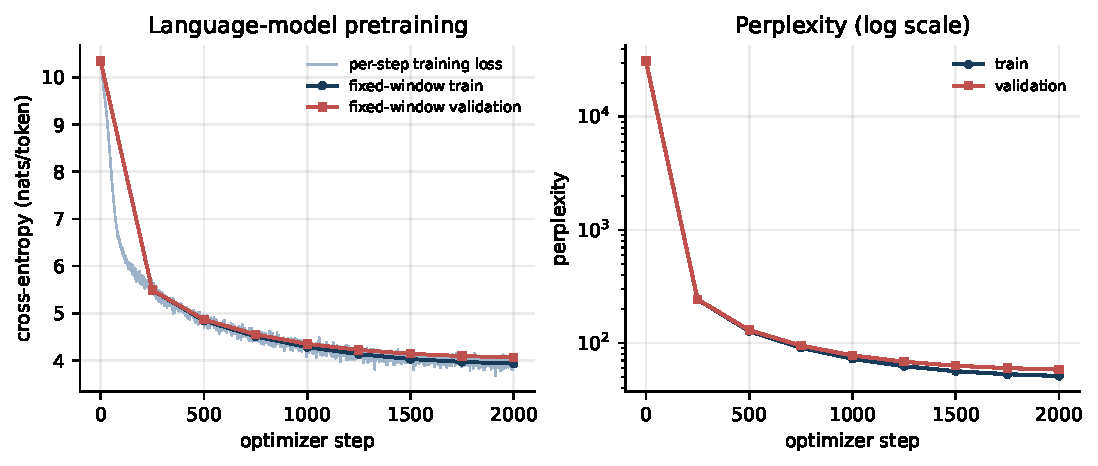
\includegraphics[width=0.96\textwidth]{figures/lm_pretraining.pdf}
\caption{AG News 语言模型预训练：逐步训练损失、固定窗口训练/验证损失和困惑度。}
\label{fig:lm}
\end{figure}

\subsection{分类器训练过程与测试结果}
表~\ref{tab:history} 记录三种解码器分类设置的逐 epoch 结果。
全参数微调第 1 个 epoch 验证准确率达到 91.67\%，第 3 个 epoch 为 93.50\%；
随机初始化从 90.69\% 起步，最终达到 92.25\%，说明 10.89M 参数的解码器从零训练
也能在 108k 条 AG News 上取得较好结果；预训练带来约 1.4 个百分点的测试准确率
提升。冻结主干的线性探针从 87.28\% 升至 87.95\%，6 个 epoch 后基本饱和。

\begin{table}[htbp]
\centering\small
\caption{解码器分类器逐 epoch 训练/验证结果}\label{tab:history}
\begin{tabular}{llrrr}
\toprule
设置 & Epoch & 训练损失 & 验证损失 & 验证准确率(\%) \\
\midrule
全参数微调 & 1 & 0.3205 & 0.2490 & 91.67 \\
全参数微调 & 2 & 0.1959 & 0.2040 & 93.31 \\
全参数微调 & 3 & 0.1476 & 0.2048 & 93.50 \\
冻结主干 & 1 & 0.5025 & 0.3673 & 87.28 \\
冻结主干 & 2 & 0.3781 & 0.3574 & 87.60 \\
冻结主干 & 3 & 0.3751 & 0.3527 & 87.80 \\
冻结主干 & 4 & 0.3725 & 0.3501 & 87.85 \\
冻结主干 & 5 & 0.3699 & 0.3498 & 87.92 \\
冻结主干 & 6 & 0.3669 & 0.3491 & 87.95 \\
随机初始化 & 1 & 0.4412 & 0.2730 & 90.69 \\
随机初始化 & 2 & 0.2211 & 0.2396 & 92.17 \\
随机初始化 & 3 & 0.1766 & 0.2499 & 92.25 \\
\bottomrule

\end{tabular}
\end{table}

全参数微调在测试集上取得 \FullAcc\% 准确率、\FullFOne\% 宏 F1、测试损失
\FullLoss，最佳 epoch 为 \FullBestEpoch。表~\ref{tab:perclass} 给出逐类指标，
图~\ref{fig:confusion} 给出混淆矩阵。Sports 的 F1 最高（97.89\%）；
Business 与 Sci/Tech 之间存在混淆，主要来自公司、产品、互联网商业新闻的
主题重叠。

\begin{table}[htbp]
\centering\small
\caption{全参数微调分类器的测试集逐类指标（\%）}\label{tab:perclass}
\begin{tabular}{lrrrr}
\toprule
类别 & 精确率 & 召回率 & F1 & 支持数 \\
\midrule
World & 93.73 & 93.68 & 93.71 & 1,900 \\
Sports & 97.10 & 98.68 & 97.89 & 1,900 \\
Business & 91.92 & 89.16 & 90.52 & 1,900 \\
Sci/Tech & 90.14 & 91.42 & 90.78 & 1,900 \\
\bottomrule

\end{tabular}
\end{table}

\begin{figure}[htbp]
\centering
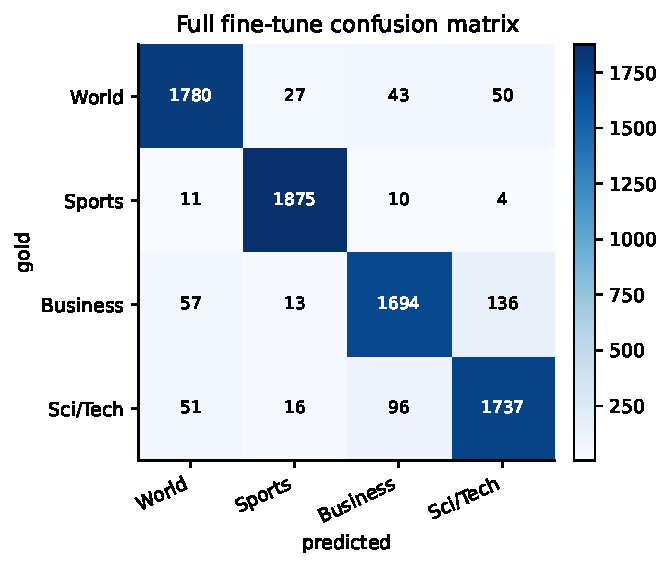
\includegraphics[width=0.55\textwidth]{figures/confusion_full.pdf}
\caption{全参数微调分类器在 AG News 测试集上的混淆矩阵。}
\label{fig:confusion}
\end{figure}

\subsection{朴素贝叶斯与 Prompt 结果}
NB 在验证集上选择 $\alpha=\NBAlpha$，使用 \NBFeatures{} 个 unigram/bigram 特征，
测试准确率 \NBAcc\%、宏 F1 \NBFOne\%，与 sklearn 实现的测试预测一致率
\NBCrossAgreement\%，说明手写的平滑、先验和判别公式与标准实现数值一致。
NB 的特征构建加拟合共耗时 \NBTrainSeconds{} 秒，其中特征提取
\NBFeatureSeconds{} 秒；测试集推理耗时 \NBInferSeconds{} 秒。
表~\ref{tab:nbtop} 展示各类别判别力最强的 n-gram。NB 会利用 Reuters 模板、
网站模板等数据集伪影（如 \code{fullquote}、\code{jhtml}），这是词袋模型在
高维稀疏文本上的典型行为；神经模型可以从上下文组合中学习。

\begin{table}[htbp]
\centering\small
\caption{多项式 NB 各类别 top-6 判别特征（对数概率差）}\label{tab:nbtop}
\begin{tabular}{lp{0.72\textwidth}}
\toprule
类别 & 代表性特征 \\
\midrule
World & ( canadian, arafat, hamas, gaza, militants, sadr \\
Sports & ( sports, sports network, network ), ticker ), preseason, knicks \\
Business & / fullquote, fullquote, . investor, stocks /, / quickinfo, quickinfo \\
Sci/Tech & pc world, strong \&, mozilla, cassini, ziff davis, ziff \\
\bottomrule

\end{tabular}
\end{table}

Prompt 结果对 verbalizer 和校准敏感。默认类别词、无校准的零样本准确率为
\PromptDefaultAcc\%。仅用验证集选择 verbalizer 并做 content-free 校准后，
测试准确率达到 \PromptAcc\%、宏 F1 \PromptFOne\%，验证集准确率
\PromptTunedVal\%。四样本设置降至 \PromptFewAcc\%：4 个示例占用 108 个词元的
上下文，测试文本被压缩；4 层小模型的上下文学习能力有限，示例中的类别词强化了
语言模型的词频偏置。表~\ref{tab:tuning} 给出验证集筛选阶段的前 5 组 verbalizer
组合。

\begin{table}[htbp]
\centering\small
\caption{验证集前 4,000 条上的 Prompt verbalizer 筛选前 5 名（校准后）}\label{tab:tuning}
\begin{tabular}{lc}
\toprule
World / Sports / Business / Sci-Tech & 验证准确率(\%) \\
\midrule
politics, sports, financial, computers & 72.78 \\
politics, sports, markets, computers & 71.62 \\
politics, sports, financial, technology & 70.93 \\
politics, sports, markets, technology & 70.30 \\
politics, sports, economy, computers & 66.80 \\
\bottomrule

\end{tabular}
\end{table}

\subsection{三种方案的总体对比}
表~\ref{tab:compare} 汇总测试准确率、宏 F1、可训练参数量、训练耗时和测试吞吐。
全参数微调准确率最高（\FullAcc\%），可训练参数 10.89M，训练约
\FullTrainSeconds{} 秒；随机初始化消融为 \ScratchAcc\%，预训练带来约 1.4 个
百分点增益；NB 以 0.8M 参数在 \NBTrainSeconds{} 秒内达到 \NBAcc\%；冻结主干
训练 \FrozenTrainable{} 个参数达到 \FrozenAcc\%，适合算力有限、需要轻量训练的
场景；Prompt 零样本无可训练参数，校准后达到 \PromptAcc\%，比监督方案低约
20 个百分点。

\begin{table}[htbp]
\centering\small
\caption{AG News 测试集上的方案对比}\label{tab:compare}
\footnotesize
\begin{tabular}{lrrrrr}
\toprule
方案 & 准确率(\%) & 宏 F1(\%) & 可训练参数 & 训练耗时(s) & 测试吞吐(样本/s) \\
\midrule
全参数微调 & 93.24 & 93.22 & 10,889,732 & 94.68 & 11,990 \\
随机初始化 & 91.86 & 91.83 & 10,889,732 & 94.34 & 12,191 \\
朴素贝叶斯 & 90.57 & 90.53 & 800,004 & 6.85 & 27,102 \\
冻结主干 & 88.03 & 88.02 & 1,028 & 71.75 & 12,296 \\
Prompt 零样本 & 73.24 & 72.94 & 0（冻结 10.89M） & 0 & 2,468 \\
Prompt 四样本 & 63.57 & 60.20 & 0（冻结 10.89M） & 0 & 1,570 \\
\bottomrule

\end{tabular}
\end{table}

\begin{figure}[htbp]
\centering
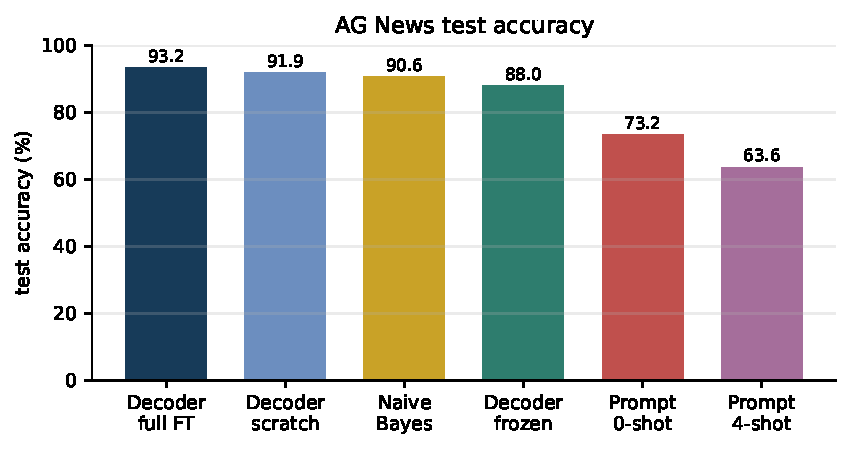
\includegraphics[width=0.78\textwidth]{figures/comparison.pdf}
\caption{各方案在 AG News 测试集上的准确率对比。}
\label{fig:compare}
\end{figure}

\begin{figure}[htbp]
\centering
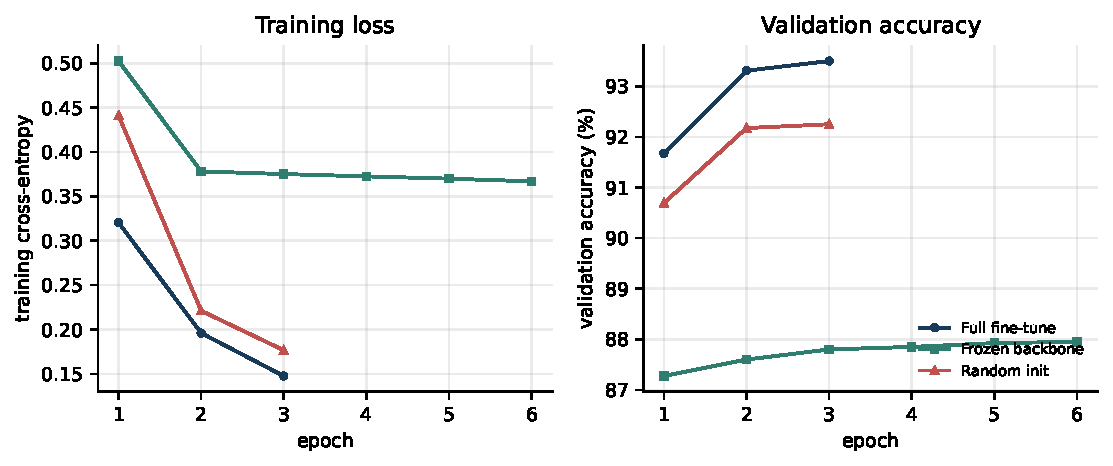
\includegraphics[width=0.96\textwidth]{figures/classifier_curves.pdf}
\caption{解码器分类器的训练损失与验证准确率曲线。冻结主干训练 6 个 epoch，
其余设置训练 3 个 epoch。}
\label{fig:cls-curves}
\end{figure}

\subsection{样例输出}
表~\ref{tab:samples} 列出 3 组固定测试样本的预测。样本 37 为 World，
零样本 Prompt 预测为 Business；样本 41 为 Business，NB 预测为 Sci/Tech；
样本 397 为 Sci/Tech，全参数微调预测为 Business，NB 与 Prompt 预测正确。
三组样本分别体现 Prompt、NB 和全参数微调的典型错误。

\begin{table}[htbp]
\centering\small
\caption{3 组测试样本的模型预测}\label{tab:samples}
\begin{tabular}{clccccc}
\toprule
索引 & 金标准 & 全参数 & 贝叶斯 & Prompt 0-shot & 冻结 & Prompt 4-shot \\
\midrule
37 & World & World & World & Business & Sci/Tech & Business \\
41 & Business & Business & Sci/Tech & Business & Sci/Tech & Sci/Tech \\
397 & Sci/Tech & Business & Sci/Tech & Sci/Tech & Sci/Tech & Sci/Tech \\
\bottomrule

\end{tabular}
\end{table}

\newpage
\begin{CodeBlock}
=== index=37, gold=World ===
Title: 1994 Law Designed to Preserve Guard Jobs (AP)
Description: AP - A 1994 law strengthened job protections for National Guard
and Reserve troops called to active duty. Here are major provisions of the
Uniformed Services Employment and Reemployment Rights Act (USERRA).

=== index=41, gold=Business ===
Title: Retailers Vie for Back-To-School Buyers (Reuters)
Description: Reuters - Apparel retailers are hoping their back-to-school
fashions will make the grade among style-conscious teens and young adults
this fall, but it could be a tough sell, with students and parents keeping a
tighter hold on their wallets.

=== index=397, gold=Sci/Tech ===
Title: Wiretapping on the Net: Who pays?
Description: NEW YORK At first glance, it might seem like the simple extension
of a standard tool in the fight against the bad guys. But in fact,
wiretapping Internet phones to monitor criminals and terrorists is costly
\end{CodeBlock}

\section{程序调试过程}

实验过程中修复了以下问题，结果均为修复后重跑所得。

\begin{enumerate}
  \item \textbf{scratch 模式误加载预训练权重}。首次运行随机初始化消融时，
        指标与全参数微调完全相同；检查发现 \code{load_lm_checkpoint} 无条件
        返回预训练 \code{backbone}，scratch 分支只改了打印信息。修复为在 scratch
        模式下重新构造 \code{DecoderLM(lm_config)}，跳过 \code{state_dict} 加载；
        重跑后测试准确率从 \FullAcc\% 变为 \ScratchAcc\%。
  \item \textbf{few-shot 与 zero-shot 指标相同}。Prompt 的 few-shot 前缀有
        178 个词元，测试前缀又按完整预算构造，超长后代码回退为只保留测试前缀，
        示例被丢弃。修复为
        \code{test_budget = budget - reserve - len(shots_prefix)}，并把示例
        正文限制在 24 个词元；四样本提示降为 108 个词元，重跑后
        few-shot 从 \PromptDefaultAcc\% 变为 \PromptFewAcc\%。
  \item \textbf{Prompt 打分显存过大}。最初对整段序列接输出头，得到
        $[B,L,V]$ 的 logits（约 2.3 GiB），再算 log-softmax 接近 OOM。
        改为只收集标签位置的隐状态，再用 \code{lm_head} 得到 $[N_{\text{label}},V]$
        的 logits；显存和计算量都显著下降。
  \item \textbf{确定性模式 cuBLAS 报错}。开启
        \code{torch.use_deterministic_algorithms(True)} 后，GPU 矩阵乘报
        “operation is not deterministic ... \code{CUBLAS_WORKSPACE_CONFIG}”。
        在导入 CUDA 相关计算前设置
        \code{CUBLAS_WORKSPACE_CONFIG=:4096:8}，并把该设置写入
        \code{src/utils.py}，脚本会自动设置该变量，保证实验可复现。
  \item \textbf{训练计时被嵌套上下文覆盖}。最初 \code{Stopwatch} 在
        \code{log_evaluation} 内部再次 \code{__enter__}，把外层起始时间覆盖，
        导致 2,000 步训练只记录 5.5 秒，逐步日志的 elapsed 字段保持不变。
        修复为带 depth 的嵌套计时，并新增 \code{current()} 供上下文内部写日志；
        重跑后预训练计时为 \LMTrainSeconds{} 秒。
  \item \textbf{参数统计 KeyError}。\code{parameter_report} 去重时只给首个
        参数建了 \code{aliases} 列表，遇到共享的 \code{lm_head.weight} 时访问
        不存在的键。修复为初始化 \code{aliases: []}，并用测试覆盖共享参数计数。
  \item \textbf{分词器 decode 丢弃 \code{<unk>}}。原实现跳过所有特殊词元，
        词表外输入在回显时消失，不便于排查 Prompt 词表问题。修复为只跳过
        pad/bos/eos，保留 \code{<unk>}；对应单元测试覆盖。
  \item \textbf{测试发现的接口问题}。\code{collate_classification} 的返回顺序为
        \code{input_ids}、\code{lengths}、\code{labels}；测试最初按
        \code{input_ids}、\code{labels}、\code{lengths} 解包，导致标签断言失败，
        修正测试后训练循环与数据接口一致。另一个测试发现 \code{min_freq}
        过滤后低频词不在 \code{stoi} 中，改为检查未知词映射到 \code{<unk>}。
\end{enumerate}

\section{分析讨论}

\subsection{效果与参数效率}
在相同数据划分上，全参数微调（\FullAcc\%）比随机初始化（\ScratchAcc\%）高约
1.4 个百分点，说明语言模型预训练提供了可迁移的词义、搭配和主题线索；
AG News 本身较容易，10.89M 参数的有监督分类器从零训练也能达到 \ScratchAcc\%。
NB 以 800,004 个对数概率参数达到 \NBAcc\%，参数效率高于神经模型；其错误主要
来自词袋丢失语序和上下文，以及 Reuters 模板等伪影。冻结主干训练 \FullHead{}
个参数得到 \FrozenAcc\%，说明预训练表示适合线性探针；全参数微调再提升约 5.2 个
百分点，代价是 10,888,704 个可训练参数和更高的训练成本。

\subsection{训练与推理开销}
全参数微调 3 个 epoch 约 \FullTrainSeconds{} 秒，测试吞吐约
\FullThroughput{} 样本/秒；NB 的特征提取加拟合约 \NBTrainSeconds{} 秒，
测试吞吐约 \NBThroughput{} 样本/秒，绝对精度低约 2.7 个百分点。
Prompt 每个测试样本前向 4 次（四个类别候选），吞吐约
\PromptThroughput{} 样本/秒，折算约 9,800 次前向/秒；Prompt 无需训练，
适合无标注、快速探索类别的场景。
冻结主干训练 6 个 epoch 约 \FrozenTrainSeconds{} 秒，单 epoch 成本低于
全参数微调，但需要更多 epoch 使线性头收敛。

\subsection{数据量需求与零样本能力}
NB 依赖类别内的词频统计，结果受特征质量影响较大。从现有结果看，全参数微调
用 108k 条带标签数据达到 \FullAcc\%，冻结主干仅训练 1,028 个分类头参数达到
\FrozenAcc\%，说明预训练表示适合线性探针且适配成本低；Prompt 零样本不使用标签，
校准后达到 \PromptAcc\%，比监督方案低约 20 个百分点。四样本 Prompt 低于零样本，
原因包括 4 层模型的上下文学习能力有限，以及示例占用上下文压缩测试文本。

默认的
\code{world} / \code{sports} / \code{business} / \code{science} 仅达到
\PromptDefaultAcc\%，验证集选出的
\code{politics} / \code{sports} / \code{financial} / \code{computers} 加 content-free
校准后达到 \PromptAcc\%。零样本仍需选择类别词，类别词的先验偏置会显著影响结果。
校准仅使用无标签模板，verbalizer 仅在验证集上选择。

\subsection{局限性与改进方向}
\begin{itemize}
  \item 采用单个随机种子和单次划分，未估计多种子置信区间；测试集 7,600 条，
        准确率标准误约 0.3 个百分点，方案间 1--2 个百分点的差异仍需重复实验
        验证。
  \item 语言模型为 4 层、$d=256$，Prompt 的 few-shot 能力受模型规模限制，
        扩大模型规模是直接改进方向。
  \item 分类器使用最后一个词元，长文本信息集中在单个词元表示中；平均池化、
        注意力池化或层级池化是自然的改进方向。
  \item NB 使用原始 Reuters 模板和 URL 片段，词袋模型会利用数据集伪影；
        更严格的文本清洗可作为后续对照。
  \item Prompt 的 verbalizer 搜索在验证集前 4,000 条上完成，存在选择偏差；
        更可靠的做法是嵌套交叉验证或使用独立开发集。
\end{itemize}

\section{结论}
本实验在作业二手写解码器上完成 AG News 文本分类。全参数微调分类头取得
\FullAcc\% 的测试准确率，为最优方案；随机初始化同结构模型为 \ScratchAcc\%，
预训练带来约 1.4 个百分点的增益；多项式 NB 以 0.8M 参数达到 \NBAcc\%，
是强基线；冻结主干的线性探针训练 \FullHead{} 个参数达到 \FrozenAcc\%，
验证了预训练表示适合线性探针；Prompt 零样本在验证集上选择 verbalizer 并做
content-free 校准后达到 \PromptAcc\%，无可训练参数，但明显落后于监督方案。
在中等规模英文新闻分类上，朴素贝叶斯仍是强基线，解码器微调的优势主要来自
上下文表示和预训练迁移；Prompt 适合无标注、快速探索的场景，精度低于有监督
微调。

\begin{thebibliography}{9}
\bibitem{zhang2015} Zhang, X., Zhao, J., LeCun, Y. Character-level convolutional
networks for text classification. \emph{Advances in Neural Information Processing
Systems}, 2015. 数据镜像：
\url{https://github.com/mhjabreel/CharCnn_Keras/tree/master/data/ag_news_csv}.
\bibitem{vaswani2017} Vaswani, A., et al. Attention is all you need.
\emph{NeurIPS}, 2017.
\bibitem{radford2019} Radford, A., et al. Language models are unsupervised
multitask learners. OpenAI technical report, 2019.
\bibitem{pedregosa2011} Pedregosa, F., et al. Scikit-learn: Machine learning in
Python. \emph{Journal of Machine Learning Research}, 12:2825--2830, 2011.
\bibitem{zhao2021} Zhao, T., Wallace, E., Feng, S., Klein, D., Singh, S.
Calibrate before use: Improving few-shot performance of language models.
\emph{ICML}, 2021.
\end{thebibliography}

\end{document}
